 %% Copyright (C) 2011, Andrea Cimino, All Rights Reserved.
 %% This file is distributed under the terms of the Creative Commons
 %% Licence Non-Commercial Share-Alike license

%% Useful stuff for separate compilation.
\ifx\ismaindoc\undefined
\providecommand{\inbpdocument}{
 \documentclass[11pt,a4paper,twoside,titlepage]{scrbook}
%%%%%%%%%%%%%%%%%%%%%%%%%%%%%%%%
%%%%%%%%%%% PACKAGES %%%%%%%%%%%
%%%%%%%%%%%%%%%%%%%%%%%%%%%%%%%%
% encoding
\usepackage[utf8x]{inputenc}
\usepackage[italian]{babel} % babel (suddivisione parole in sillabe)

\usepackage{amsfonts} % matematica
\usepackage{amsmath} % matematica
\usepackage{amssymb} % simboli vari
\usepackage{calrsfs}
\usepackage{caption}
\usepackage{enumerate}
\usepackage{extarrows} % matematica
\usepackage{keyval}
\usepackage{manfnt} % Simboli curva
\usepackage{mathtools} % matematica
\usepackage{multirow} 
\usepackage[usenames, dvipsnames]{color} % colori con nome
\usepackage[pdftex]{graphicx}
\usepackage{epstopdf} % gestione file EPS
\usepackage{wrapfig} % per figure circondate da testo
\usepackage{framed}	% teoremi framed
\usepackage{fancyhdr} % header buffi
\usepackage[T1]{fontenc} % gestione hbox e vbox
\usepackage[a4paper]{geometry}
\usepackage{microtype} % gestione hbox e vbox
\usepackage[thref, amsthm, amsmath, framed, hyperref]{ntheorem} % teoremi (avanzata)
%% \usepackage{prooftree} % gestione prof-tree
\usepackage{rotating}
\usepackage{stmaryrd}
\usepackage{subfig}
\usepackage{syntax} % syntattic stuff
\usepackage{txfonts}
\usepackage{verbatim} % migliorie al verbatim
%\usepackage{hyperref}
%% \usepackage{qtree}
\usepackage{fancyvrb}
\usepackage{listings}
\usepackage{cancel}
\usepackage{tikz}

\usepackage{bbding} %% Icons

%%%%%%%%%%%%%%%%%%%%%%%%%%%%%%%%
%%%%%%%%%%% GEOMETRY %%%%%%%%%%%
%%%%%%%%%%%%%%%%%%%%%%%%%%%%%%%%
\geometry{verbose,tmargin=2cm,bmargin=2.5cm,lmargin=2.5cm,rmargin=2cm}
\parindent0ex %% Remove paragraph indenting

%%%%%%%%%%%%%%%%%%%%%%%%%%%%%%%%
%%%%%%%%%%% CODE ENV %%%%%%%%%%%
%%%%%%%%%%%%%%%%%%%%%%%%%%%%%%%%
% codice
\newcounter{count}
\setcounter{count}{0}
\newenvironment{code}[1]
{
\color{lightgray}\hrulefill\color{code}
\stepcounter{count} {\bf\small Listato di codice \arabic{count}: {#1} }
\verbatim
}
{
\endverbatim
\color{lightgray}\hrulefill
\color{black}
\\
}

% codice semplice
\newenvironment{simplecode}
{
\color{code} \tt
}
{
\rm
}

 % Notation issues

%% Proof trees.
%\input prooftree
\newcommand*{\nohyp}{\phantom{x}}

%% C++.
\newcommand*{\Cplusplus}{{C\nolinebreak[4]\hspace{-.05em}\raisebox{.4ex}
{\tiny\bf ++}}}

%% BNF rules.
\newcommand*{\vbar}{\mathrel{\mid}}

%% Abstract syntax of the analyzed language.
\newcommand*{\Type}{\mathrm{Type}}
\newcommand*{\dType}{\mathrm{dType}}
\newcommand*{\dT}{\mathrm{dT}}
\newcommand*{\sType}{\mathrm{sType}}
\newcommand*{\sT}{\mathrm{sT}}
\newcommand*{\cType}{\mathrm{cType}}
\newcommand*{\cT}{\mathrm{cT}}
\newcommand*{\Integer}{\mathrm{Integer}}
\newcommand*{\Bool}{\mathrm{Bool}}
\newcommand*{\Id}{\mathrm{Id}}
\newcommand*{\id}{\mathrm{id}}
\newcommand*{\rId}{\mathrm{rId}}
\newcommand*{\idx}{\mathrm{x}}
\newcommand*{\ridx}{\underline{\mathrm{x}}}
\newcommand*{\Exp}{\mathrm{Exp}}
\newcommand*{\Exps}{\mathrm{Exps}}
\newcommand*{\Decl}{\mathrm{Decl}}
\newcommand*{\exceptDecl}{\mathrm{exceptDecl}}
\newcommand*{\Catch}{\mathrm{Catch}}
\newcommand*{\Stmt}{\mathrm{Stmt}}
\newcommand*{\Label}{\mathrm{Label}}
\newcommand*{\Con}{\mathrm{Con}}
\newcommand*{\con}{\mathrm{con}}
\newcommand*{\fps}{\mathrm{fps}}
\newcommand*{\funBody}{\mathrm{Body}}
\newcommand*{\funbody}{\mathrm{body}}
\newcommand*{\main}{\mathrm{main}}
\newcommand*{\es}{\mathrm{es}}
\newcommand*{\formParams}{\mathrm{formParams}}
\newcommand*{\emptysequence}{\boxempty}
\newcommand*{\Glob}{\mathrm{Glob}}

%% Sets of configurations
\newcommand*{\NTe}{\Gamma_\mathrm{e}}
\newcommand*{\NTb}{\Gamma_\mathrm{b}}
\newcommand*{\NTd}{\Gamma_\mathrm{d}}
\newcommand*{\NTg}{\Gamma_\mathrm{g}}
\newcommand*{\NTs}{\Gamma_\mathrm{s}}
\newcommand*{\NTk}{\Gamma_\mathrm{k}}
\newcommand*{\Te}{T_\mathrm{e}}
\newcommand*{\Tb}{T_\mathrm{b}}
\newcommand*{\Td}{T_\mathrm{d}}
\newcommand*{\Tg}{T_\mathrm{g}}
\newcommand*{\Ts}{T_\mathrm{s}}
\newcommand*{\Tk}{T_\mathrm{k}}

%% Lambda notation.
\newcommand*{\lambdaop}{\mathop{\lambda}\nolimits}

%% Sets of (no better specified) configurations.
\newcommand*{\NT}[1]{\Gamma_{#1}}
\newcommand*{\NTq}{\Gamma_q}
\newcommand*{\Tq}{T_q}

%% Denotable values.
\newcommand*{\dVal}{\mathrm{dVal}}
%% Storeable values.
\newcommand*{\sVal}{\mathrm{sVal}}
\newcommand*{\sval}{\mathrm{sval}}

%% Control modes.
\newcommand*{\CtrlMode}{\mathord{\mathrm{CtrlMode}}}
\newcommand*{\cm}{\mathrm{cm}}
%% Branch modes.
%\newcommand*{\BranchMode}{\mathord{\mathrm{BranchMode}}}
\newcommand*{\GotoMode}{\mathord{\mathrm{GotoMode}}}
\newcommand*{\SwitchMode}{\mathord{\mathrm{SwitchMode}}}
\newcommand*{\cmgoto}{\mathop{\mathrm{goto}}\nolimits}
\newcommand*{\cmswitch}{\mathop{\mathrm{switch}}\nolimits}
\newcommand*{\cmbreak}{\mathop{\mathrm{break}}\nolimits}
\newcommand*{\cmcontinue}{\mathop{\mathrm{continue}}\nolimits}
\newcommand*{\cmreturn}{\mathop{\mathrm{return}}\nolimits}
%% Exec mode.
\newcommand*{\cmexec}{\mathrm{exec}}
%% Value mode.
\newcommand*{\ValMode}{\mathord{\mathrm{ValMode}}}
\newcommand*{\cmvalue}{\mathop{\mathrm{value}}\nolimits}
%% Environment mode.
\newcommand*{\EnvMode}{\mathord{\mathrm{EnvMode}}}
\newcommand*{\cmenv}{\mathrm{env}}
%% Exception modes.
\newcommand*{\ExceptMode}{\mathord{\mathrm{ExceptMode}}}
\newcommand*{\cmexcept}{\mathrm{except}}

%% Control states.
\newcommand*{\CtrlState}{\mathord{\mathrm{CtrlState}}}
\newcommand*{\cs}{\mathord{\mathrm{cs}}}
%% Value states.
\newcommand*{\ValState}{\mathord{\mathrm{ValState}}}
\newcommand*{\valstate}{\upsilon}
%% Environment states.
%\newcommand*{\EnvState}{\mathord{\mathrm{EnvState}}}
%% Exception states.
\newcommand*{\ExceptState}{\mathord{\mathrm{ExceptState}}}
\newcommand*{\exceptstate}{\varepsilon}

%% Keywords.
\newcommand*{\kw}[1]{\mathop{\textup{\textbf{#1}}}}

\newcommand*{\bop}{\mathbin{\mathrm{bop}}}
%\newcommand*{\uop}{\mathop{\mathrm{uop}}}

%% Things that hold by definition.
\newcommand{\defrel}[1]{\mathrel{\buildrel \mathrm{def} \over {#1}}}
\newcommand{\defeq}{\defrel{=}}
\newcommand{\defiff}{\defrel{\Longleftrightarrow}}
%\newcommand{\defeq}{=}
%\newcommand{\defiff}{\Longleftrightarrow}

%% Divergence relation
\newcommand{\diverges}{\,\mathord{\buildrel \infty \over \longrightarrow}}

%% Special letters denoting sets and algebras.
\providecommand*{\Nset}{\mathbb{N}}             % Naturals
\providecommand*{\Qset}{\mathbb{Q}}             % Rationals
\providecommand*{\Zset}{\mathbb{Z}}             % Integers
\providecommand*{\Rset}{\mathbb{R}}             % Reals

%% Calligraphic alphabet.
\newcommand*{\calA}{\ensuremath{\mathcal{A}}}
\newcommand*{\calB}{\ensuremath{\mathcal{B}}}
\newcommand*{\calC}{\ensuremath{\mathcal{C}}}
\newcommand*{\calD}{\ensuremath{\mathcal{D}}}
\newcommand*{\calE}{\ensuremath{\mathcal{E}}}
\newcommand*{\calF}{\ensuremath{\mathcal{F}}}
\newcommand*{\calG}{\ensuremath{\mathcal{G}}}
\newcommand*{\calH}{\ensuremath{\mathcal{H}}}
\newcommand*{\calI}{\ensuremath{\mathcal{I}}}
\newcommand*{\calJ}{\ensuremath{\mathcal{J}}}
\newcommand*{\calK}{\ensuremath{\mathcal{K}}}
\newcommand*{\calL}{\ensuremath{\mathcal{L}}}
\newcommand*{\calM}{\ensuremath{\mathcal{M}}}
\newcommand*{\calN}{\ensuremath{\mathcal{N}}}
\newcommand*{\calO}{\ensuremath{\mathcal{O}}}
\newcommand*{\calP}{\ensuremath{\mathcal{P}}}
\newcommand*{\calQ}{\ensuremath{\mathcal{Q}}}
\newcommand*{\calR}{\ensuremath{\mathcal{R}}}
\newcommand*{\calS}{\ensuremath{\mathcal{S}}}
\newcommand*{\calT}{\ensuremath{\mathcal{T}}}
\newcommand*{\calU}{\ensuremath{\mathcal{U}}}
\newcommand*{\calV}{\ensuremath{\mathcal{V}}}
\newcommand*{\calW}{\ensuremath{\mathcal{W}}}
\newcommand*{\calX}{\ensuremath{\mathcal{X}}}
\newcommand*{\calY}{\ensuremath{\mathcal{Y}}}
\newcommand*{\calZ}{\ensuremath{\mathcal{Z}}}

%% Declarators for functions and relations.
\newcommand*{\reld}[3]{\mathord{#1}\subseteq#2\times#3}
\newcommand*{\fund}[3]{\mathord{#1}\colon#2\to#3}
\newcommand*{\pard}[3]{\mathord{#1}\colon#2\rightarrowtail#3}

%% Logical quantifiers stuff.
\newcommand{\st}{\mathrel{.}}
\newcommand{\itc}{\mathrel{:}}

%% Domain, codomain and range of a function.
\newcommand*{\dom}{\mathop{\mathrm{dom}}\nolimits}
%\newcommand*{\cod}{\mathop{\mathrm{cod}}\nolimits}
%\newcommand*{\range}{\mathop{\mathrm{range}}\nolimits}

%% Restriction of a function.
\newcommand*{\restrict}[1]{\mathop{\mid}\nolimits_{#1}}

%% Type of a constant.
\newcommand*{\type}{\mathop{\mathrm{type}}\nolimits}

%% Lubs, glbs, and fixed points.
\newcommand*{\lub}{\mathop{\mathrm{lub}}\nolimits}
%\newcommand*{\glb}{\mathop{\mathrm{glb}}\nolimits}
\newcommand*{\lfp}{\mathop{\mathrm{lfp}}\nolimits}
\newcommand*{\gfp}{\mathop{\mathrm{gfp}}\nolimits}

%% Generic widening.
\newcommand*{\widen}{\mathbin{\nabla}}

%% Set theory.
\renewcommand{\emptyset}{\varnothing}

%\newcommand*{\wpc}{\mathop{\wp_\mathrm{c}}\nolimits}
%\newcommand*{\wpf}{\mathop{\wp_\mathrm{f}}\nolimits}
%\newcommand*{\wpn}{\mathop{\wp_\mathrm{n}}\nolimits}

\newcommand*{\sseq}{\subseteq}
\newcommand*{\sseqf}{\mathrel{\subseteq_\mathrm{f}}}
\newcommand*{\sslt}{\subset}
%\newcommand*{\Sseq}{\supseteq}
%\newcommand*{\Ssgt}{\supset}

%\newcommand{\Nsseq}{\nsubseteq}

\newcommand*{\union}{\cup}
\newcommand*{\bigunion}{\bigcup}
%\newcommand*{\biginters}{\bigcap}
\newcommand*{\inters}{\cap}
\newcommand*{\setdiff}{\setminus}

\newcommand{\sset}[2]{{\renewcommand{\arraystretch}{1.2}
                      \left\{\,#1 \,\left|\,
                               \begin{array}{@{}l@{}}#2\end{array}
                      \right.   \,\right\}}}

%% Base sets.
\newcommand*{\ttv}{\mathrm{tt}}
\newcommand*{\ffv}{\mathrm{ff}}
\newcommand*{\divop}{\mathbin{/}}
\newcommand*{\modop}{\mathbin{\%}}
\newcommand*{\andop}{\mathbin{\textbf{\textup{and}}}}
\newcommand*{\orop}{\mathbin{\textbf{\textup{or}}}}
\newcommand*{\notop}{\mathop{\textbf{\textup{not}}}}

\newcommand*{\FI}{\mathop{\mathrm{FI}}\nolimits}
\newcommand*{\DI}{\mathop{\mathrm{DI}}\nolimits}
\newcommand*{\SL}{\mathop{\mathrm{SL}}\nolimits}
%\newcommand*{\match}{\mathop{\mathrm{match}}\nolimits}

\newcommand*{\Env}{\mathord{\mathrm{Env}}}
\newcommand*{\emptystring}{\mathord{\epsilon}}

%% Exceptions.
\newcommand*{\RTSExcept}{\mathord{\mathrm{RTSExcept}}}
\newcommand*{\rtsexcept}{\chi}
\newcommand*{\Except}{\mathord{\mathrm{Except}}}
\newcommand*{\except}{\xi}
\newcommand*{\none}{\mathtt{none}}
\newcommand*{\divbyzero}{\mathtt{divbyzero}}
\newcommand*{\stkovflw}{\mathtt{stkovflw}}
\newcommand*{\datovflw}{\mathtt{datovflw}}
\newcommand*{\memerror}{\mathtt{memerror}}
%\newcommand*{\inerror}{\mathtt{inerror}}
%\newcommand*{\nullptr}{\mathtt{nullptr}}
%\newcommand*{\outofboundsptr}{\mathtt{outofboundsptr}}

%% Flags for terminal configurations of catch clauses.
\newcommand*{\caught}{\mathtt{caught}}
\newcommand*{\uncaught}{\mathtt{uncaught}}

%% Static semantics.
\newcommand*{\TEnv}{\mathord{\mathrm{TEnv}}}
\newcommand*{\tinteger}{\mathrm{integer}}
\newcommand*{\tboolean}{\mathrm{boolean}}
\newcommand*{\trtsexcept}{\mathrm{rts\_exception}}

%% Memory structures.
\newcommand*{\Loc}{\mathord{\mathrm{Loc}}}
\newcommand*{\Ind}{\mathrm{Ind}}
\newcommand*{\Addr}{\mathrm{Addr}}
\newcommand*{\Map}{\mathrm{Map}}
%\newcommand*{\eMap}{\mathrm{eMap}}
\newcommand*{\Stack}{\mathord{\mathrm{Stack}}}
\newcommand*{\Mem}{\mathord{\mathrm{Mem}}}
\newcommand*{\stknew}{\mathop{\mathrm{new}_\mathrm{s}}\nolimits}
\newcommand*{\datnew}{\mathop{\mathrm{new}_\mathrm{d}}\nolimits}
\newcommand*{\txtnew}{\mathop{\mathrm{new}_\mathrm{t}}\nolimits}
\newcommand*{\heapnew}{\mathop{\mathrm{new}_\mathrm{h}}\nolimits}
\newcommand*{\heapdel}{\mathop{\mathrm{delete}_\mathrm{h}}\nolimits}
\newcommand*{\datcleanup}{\mathop{\mathrm{cleanup}_\mathrm{d}}\nolimits}
\newcommand*{\smark}{\mathop{\mathrm{mark}_\mathrm{s}}\nolimits}
\newcommand*{\sunmark}{\mathop{\mathrm{unmark}_\mathrm{s}}\nolimits}
\newcommand*{\slink}{\mathop{\mathrm{link}_\mathrm{s}}\nolimits}
\newcommand*{\sunlink}{\mathop{\mathrm{unlink}_\mathrm{s}}\nolimits}
\newcommand*{\asmark}{\mathop{\mathrm{mark}_\mathrm{s}^\sharp}\nolimits}
\newcommand*{\asunmark}{\mathop{\mathrm{unmark}_\mathrm{s}^\sharp}\nolimits}
\newcommand*{\aslink}{\mathop{\mathrm{link}_\mathrm{s}^\sharp}\nolimits}
\newcommand*{\asunlink}{\mathop{\mathrm{unlink}_\mathrm{s}^\sharp}\nolimits}
\newcommand*{\aswiden}{\mathop{\mathrm{widen}}\nolimits}
\newcommand*{\sm}{\dag}
\newcommand*{\fm}{\ddag}
\newcommand*{\topmost}{\mathop{\mathrm{tf}}\nolimits}
%% Short forms of \datcleanup, \sunmark, \sunlink for table.
\newcommand*{\datcleanupshort}{\mathop{\mathrm{cu}_\mathrm{d}}\nolimits}
\newcommand*{\sunmarkshort}{\mathop{\mathrm{um}_\mathrm{s}}\nolimits}
\newcommand*{\sunlinkshort}{\mathop{\mathrm{ul}_\mathrm{s}}\nolimits}

\newcommand*{\location}[1]{\mathord{#1 \; \mathrm{loc}}}
%\newcommand*{\saeval}{\mathop{\mathrm{aeval}}\nolimits}
%\newcommand*{\saupd}{\mathop{\mathrm{aupd}}\nolimits}
\newcommand*{\asupported}{\mathop{\mathrm{supported}^\sharp}\nolimits}
\newcommand*{\aeval}{\mathop{\mathrm{eval}^\sharp}\nolimits}
\newcommand*{\ceval}[1]{\mathop{\mathrm{eval}_{#1}}\nolimits}

%% Abstracts.
\newcommand*{\Abstract}{\mathord{\mathrm{Abstract}}}
\newcommand*{\abs}{\mathord{\mathrm{abs}}}

%% Integer part function.
\newcommand{\intp}{\mathop{\mathrm{int}}\nolimits}

%% Concrete functions and operations.
% Aritmethic
%% \newcommand*{\conadd}{\mathbin{\boxplus}}
%% \newcommand*{\consub}{\mathbin{\boxminus}}
%% \newcommand*{\conmul}{\mathbin{\boxdot}}
%% \newcommand*{\condiv}{\mathbin{\boxslash}}
%% \newcommand*{\conmod}{\mathbin{\boxbar}}
% Boolean
%% \newcommand*{\coneq}{\mathbin{\triangleq}}
%% \newcommand*{\conineq}{\mathbin{\trianglelefteq}}
%% \newcommand*{\conneg}{\mathbin{\daleth}}
%% \newcommand*{\conor}{\mathbin{\triangledown}}
%% \newcommand*{\conand}{\mathbin{\vartriangle}}
\newcommand*{\bneg}{\mathop{\neg}\nolimits}

%% Abstract functions and operations.
% Aritmethic
\newcommand*{\absuminus}{\mathop{\ominus}\nolimits}
\newcommand*{\absadd}{\mathbin{\oplus}}
\newcommand*{\abssub}{\mathbin{\ominus}}
\newcommand*{\absmul}{\mathbin{\odot}}
\newcommand*{\absdiv}{\mathbin{\oslash}}
\newcommand*{\absmod}{\mathbin{\obar}}
% Boolean
\newcommand*{\abseq}{\mathrel{\triangleq}}
\newcommand*{\absneq}{\mathrel{\not\triangleq}}
\newcommand*{\absleq}{\mathrel{\trianglelefteq}}
\newcommand*{\abslt}{\mathrel{\vartriangleleft}}
\newcommand*{\absgeq}{\mathrel{\trianglerighteq}}
\newcommand*{\absgt}{\mathrel{\vartriangleright}}
\newcommand*{\absneg}{\mathrel{\circleddash}}
\newcommand*{\absor}{\mathrel{\ovee}}
\newcommand*{\absand}{\mathrel{\owedge}}

%% Summaries for theorem-like environments
\newcommand{\summary}[1]{\textrm{\textbf{\textup{#1}}}}

%% Filter function extracting the relevant and irrelevant parts.
\newcommand*{\sel}{\mathop{\mathrm{sel}}\nolimits}
\newcommand*{\mem}{\mathop{\mathrm{mem}}\nolimits}

%% Modeling definite exceptions.
%\newcommand*{\None}{\mathrm{None}}

%% Strict Cartesian products.
\newcommand*{\stimes}{\otimes}
\newcommand*{\spair}[2]{{#1} \otimes {#2}}
%\newcommand*{\rstimes}{\rtimes}
%\newcommand*{\rspair}[2]{{#1} \rtimes {#2}}
%\newcommand*{\lstimes}{\ltimes}
%\newcommand*{\lspair}[2]{{#1} \ltimes {#2}}

%% Additional syntax for the numeric type extension supplement
\newcommand*{\iT}{\mathrm{iT}}
\newcommand*{\iType}{\mathrm{iType}}
\newcommand*{\tschar}{\mathrm{signed\_char}}
\newcommand*{\tuchar}{\mathrm{unsigned\_char}}
\newcommand*{\flcon}{\mathrm{fl}}
\newcommand*{\Float}{\mathrm{Float}}
\newcommand*{\sccon}{\mathrm{sc}}
\newcommand*{\sChar}{\mathrm{sChar}}
\newcommand*{\uccon}{\mathrm{uc}}
\newcommand*{\uChar}{\mathrm{uChar}}

%% Additional macros for the extension for extra numeric types
%% Floating point types.
\newcommand*{\tfloat}{\mathrm{float}}
%% Numeric types
\newcommand*{\nType}{\mathrm{nType}}
\newcommand*{\nT}{\mathrm{nT}}

%% Additional macros for the extension to pointer and arrays:
%% Elementary types.
\newcommand*{\eType}{\mathrm{eType}}
\newcommand*{\eT}{\mathrm{eT}}
%% Elementary values.
%\newcommand*{\eValue}{\mathrm{eVal}}
%% Array types.
\newcommand*{\aType}{\mathrm{aType}}
\newcommand*{\aT}{\mathrm{aT}}
%% Record types.
\newcommand*{\rType}{\mathrm{rType}}
\newcommand*{\rT}{\mathrm{rT}}
%% Object types.
\newcommand*{\oType}{\mathrm{oType}}
\newcommand*{\oT}{\mathrm{oT}}
%% Function types.
\newcommand*{\fType}{\mathrm{fType}}
\newcommand*{\fT}{\mathrm{fT}}
%% Memory types.
\newcommand*{\mType}{\mathrm{mType}}
\newcommand*{\mT}{\mathrm{mT}}
%% Pointer types.
\newcommand*{\pType}{\mathrm{pType}}
\newcommand*{\pT}{\mathrm{pT}}
%% Offsets.
\newcommand*{\Offset}{\mathrm{Offset}}
\newcommand*{\nooffset}{\boxempty}
\newcommand*{\indexoffset}[1]{\mathopen{\boldsymbol{[}}{#1}\mathclose{\boldsymbol{]}}}
\newcommand*{\fieldoffset}[1]{\mathop{\boldsymbol{.}}{#1}}
%% Lvalues.
\newcommand*{\lValue}{\mathrm{LValue}}
\newcommand*{\lvalue}{\mathrm{lval}}
%% Rvalues.
\newcommand*{\rValue}{\mathrm{RValue}}
\newcommand*{\rvalue}{\mathrm{rval}}
%%
\newcommand*{\pointer}[1]{{#1}\boldsymbol{\ast}}
\newcommand*{\maddress}[1]{\mathop{\&}{#1}}
\newcommand*{\indirection}[1]{\mathop{\boldsymbol{\ast}}{#1}}
%%
\newcommand*{\locnull}{\mathord{l_\mathrm{null}}}
\newcommand*{\ptrmove}{{\mathop{\mathrm{ptrmove}}\nolimits}}
\newcommand*{\ptrdiff}{{\mathop{\mathrm{ptrdiff}}\nolimits}}
\newcommand*{\ptrcmp}{{\mathop{\mathrm{ptrcmp}}\nolimits}}
%%
\newcommand*{\arraysyntax}[3]{\kw{#1} {#2} \kw{of}\,{#3}}
\newcommand*{\arraytype}[2]{\arraysyntax{array}{#1}{#2}}
\newcommand*{\firstof}{{\mathop{\mathrm{firstof}}\nolimits}}
\newcommand*{\arrayindex}{\mathop{\mathrm{index}}\nolimits}
\newcommand*{\locindex}{\mathop{\mathrm{locindex}}\nolimits}
%%
\newcommand*{\recordsyntax}[3]{\kw{#1} {#2} \kw{of}\,{#3}}
\newcommand*{\recordtype}[2]{\recordsyntax{record}{#1}{#2}}
\newcommand*{\field}{\mathop{\mathrm{field}}\nolimits}
\newcommand*{\locfield}{\mathop{\mathrm{locfield}}\nolimits}
%%
\newcommand*{\NTo}{\Gamma_\mathrm{o}}
\newcommand*{\To}{T_\mathrm{o}}
\newcommand*{\NTl}{\Gamma_\mathrm{l}}
\newcommand*{\Tl}{T_\mathrm{l}}
%\newcommand*{\NTr}{\Gamma_\mathrm{r}}
%\newcommand*{\Tr}{T_\mathrm{r}}
%%
\newcommand*{\arraydatnew}{\mathop{\mathrm{newarray}_\mathrm{d}}\nolimits}
\newcommand*{\arraystknew}{\mathop{\mathrm{newarray}_\mathrm{s}}\nolimits}
\newcommand\Cut{\using\sf cut\thickness.08em\justifies}
\newcommand{\maybeeq}{\mathrel{\buildrel \mathrm{?} \over =}}



\makeatletter
\g@addto@macro\@verbatim\footnotesize
\makeatother



%%%%%%%%%%%%%%%%%%%%%%%%%%%%%%%%
%%%%%%%% THEOREMS FORMAT %%%%%%%
%%%%%%%%%%%%%%%%%%%%%%%%%%%%%%%%
% shaded theorems and proofs command
\definecolor{lightgray}{RGB}{230,230,230}
\def\theoremframecommand{\colorbox{lightgray}}

%%% theorems
\theoremstyle{break}
\theoremheaderfont{\normalfont\bfseries}
\theorembodyfont{\itshape}
\theoremsymbol{\ensuremath{\diamondsuit}}
\theoremseparator{\newline}
\newtheorem{theo}{
\includegraphics[scale=0.11]{imgs/book.png}Teorema}[chapter]

%%% propositions
\theoremstyle{break}
\theoremheaderfont{\normalfont\bfseries}
\theorembodyfont{\itshape}
\theoremsymbol{\ensuremath{\diamondsuit}}
\theoremseparator{\newline}
\newshadedtheorem{proposition}{Proposizione}[chapter]

%%% exercises
\theoremstyle{break}
\theoremheaderfont{\normalfont\bfseries}
\theorembodyfont{\itshape}
\theoremsymbol{\ensuremath{\diamondsuit}}
\theoremseparator{\newline}
\newshadedtheorem{exercise}{Esercizio}[chapter]

%%% propositions
\theoremstyle{break}
\theoremheaderfont{\normalfont\bfseries}
\theorembodyfont{\itshape}
\theoremsymbol{\ensuremath{\diamondsuit}}
\theoremseparator{\newline}
\newshadedtheorem{property}{\PencilRightDown $\; $ Propriet\`a}[chapter]

%%% lemmas
\theoremstyle{break}
\theoremheaderfont{\normalfont\bfseries}
\theorembodyfont{\itshape}
\theoremsymbol{\ensuremath{\diamondsuit}}
\theoremseparator{\newline}
\newshadedtheorem{lemma}[theo]{Lemma}

%%% definitions
\theoremstyle{break}
\theoremsymbol{\ensuremath{\clubsuit}}
\theoremseparator{\newline}
\newshadedtheorem{defn}[theo]{Definizione}

%%% examples
\theoremstyle{break}
\theorembodyfont{\itshape}
\theoremsymbol{\ensuremath{\ast}}
\theoremseparator{\newline}
\newshadedtheorem{example}[theo]{Esempio}

%%% observations
\theoremstyle{break}
\theorembodyfont{\itshape}
\theoremsymbol{\ensuremath{\ast}}
\theoremseparator{\newline}
\newshadedtheorem{observation}[theo]{

\includegraphics[scale=0.06]{imgs/lens.png}
Osservazione
}

%%% notations
\newtheorem*{notaz}{Notazione}

%%% proofs
\newenvironment{thproof}
{
\vskip 0.03cm
\begin{small}
\textit{Dimostrazione. }
\color{code}
}
{
\color{black}
\end{small}
$ \square $
\vskip 0.2cm
}

%Notes
\newenvironment{notes}{%
  \def\FrameCommand{\colorbox{yellow}}%
  \MakeFramed {\FrameRestore}
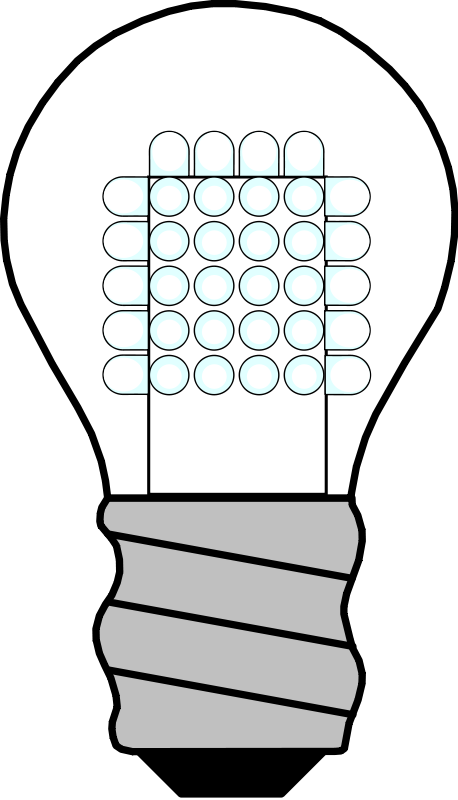
\includegraphics[scale=0.02]{imgs/bulb.png}
 \textbf{Nota} \\
 }%
{\endMakeFramed}

%Work in progress
\newenvironment{workinprogress}{%
  \def\FrameCommand{\colorbox{pink}}%
  \MakeFramed {\FrameRestore}
\lhdbend  \textbf{Work in progress} \\
 }%
{\endMakeFramed}

%Openquestion
\newenvironment{openquestion}{%
  \def\FrameCommand{\colorbox{pink}}%
  \MakeFramed {\FrameRestore}
 \textbf{Domanda aperta} \\
 }%
{\endMakeFramed}

%TODO
\newenvironment{todo}{%
  \def\FrameCommand{\colorbox{pink}}%
  \MakeFramed {\FrameRestore}
 \textbf{TODO} \\
 }%
{\endMakeFramed}

%%%%%%%%%%%%%%%%%%%%%%%%%%%%%%%%
%%%%%%%%%%%% HEADER %%%%%%%%%%%%
%%%%%%%%%%%%%%%%%%%%%%%%%%%%%%%%
\pagestyle{fancy}
% i comandi seguenti impediscono la scrittura in maiuscolo
% dei nomi dei capitoli e dei paragrafi nelle intestazioni
\renewcommand{\chaptermark}[1]{\markboth{#1}{}}
\renewcommand{\sectionmark}[1]{\markright{\thesection\ #1}}
\fancyhf{} % rimuove l'attuale contenuto dell'intestazione
% e del pi\`e di pagina
\fancyhead[LE,RO]{\bfseries\thepage}
\fancyhead[LO]{\bfseries\rightmark}
\fancyhead[RE]{\bfseries\leftmark}
\renewcommand{\headrulewidth}{0.5pt}
\renewcommand{\footrulewidth}{0pt}
\addtolength{\headheight}{0.5pt} % riserva spazio per la linea
\fancypagestyle{plain}{%
\fancyhead{} % ignora, nello stile plain, le intestazioni
\renewcommand{\headrulewidth}{0pt} % e la linea
}


%%%%%%%%%%%%%%%%%%%%%%%%%%%%%%%%
%%%%%%%%%%%% COLORS %%%%%%%%%%%%
%%%%%%%%%%%%%%%%%%%%%%%%%%%%%%%%
\definecolor{code}{gray}{0.3}


%%%%%%%%%%%%%%%%%%%%%%%%%%%%%%%%
%%%%%%%%%%%% NUMBERS %%%%%%%%%%%
%%%%%%%%%%%%%%%%%%%%%%%%%%%%%%%%
\setcounter{tocdepth}{3}
\setcounter{secnumdepth}{3}


%%%%%%%%%%%%%%%%%%%%%%%%%%%%%%%%
%%%%%%%%%%% DOC DATA %%%%%%%%%%%
%%%%%%%%%%%%%%%%%%%%%%%%%%%%%%%%
\title{Appunti di MNO}
\author{Gruppo Informatici Rampanti}
\date{ott 2010 - mag 2011}

\pdfinfo{%
  /Title    (Appunti di MNO)
  /Author   (Andrea Cimino e Lorenzo Muti)
  /Creator  (Andrea Cimino)
  /Producer (Lorenzo Muti)
  /Subject  (MNO)
  /Keywords (MNO)
}


%%%%%%%%%%%%%%%%%%%%%%%%%%%%%%%%
%%%%%%%%%%%%% UTILS %%%%%%%%%%%%
%%%%%%%%%%%%%%%%%%%%%%%%%%%%%%%%
% binary symbols
\newcommand{\modder}{\vdash _{R}}

% vertical gaps
\newcommand{\askip}{\vspace{0.5cm}}
\newcommand{\bskip}{\vspace{1.0cm}}

% various symbols
\newcommand{\qedhere}{\ensuremath{\Box}}
\newcommand{\qed}{\hfill \ensuremath{\Box}}

% substitution
\newcommand{\subst}[2]{^{#1} / _{#2}}

% denotational semantics function names
\newcommand{\bbracket}[1]{\left\llbracket #1 \right\rrbracket}

\newcommand{\aexpr}{\mathcal{A}}
\newcommand{\bexpr}{\mathcal{B}}
\newcommand{\cexpr}{\mathcal{C}}
\newcommand{\Aexpr}[1]{\mathcal{A} \bbracket{#1}}
\newcommand{\Bexpr}[1]{\mathcal{B} \bbracket{#1}}
\newcommand{\Cexpr}[1]{\mathcal{C} \bbracket{#1}}

\newcommand{\semdomset}[1]{(V_{#1})_{\bot}}

% semantic evaluations
\newcommand{\opereval}[3]{\left\langle #1, #2 \right\rangle \rightarrow #3}
\newcommand{\denaeval}[3]{\Aexpr{#1} #2 = #3}
\newcommand{\denbeval}[3]{\Bexpr{#1} #2 = #3}
\newcommand{\denceval}[3]{\Cexpr{#1} #2 = #3}

% rotated sqsubseteqs
\newcommand{\upsqsubseteq}{ $\begin{rotate}{90} $\sqsubseteq$ \end{rotate}$ }
\newcommand{\downsqsubseteq}{ $\begin{rotate}{270} $\sqsubseteq$ \end{rotate}$ }

% Space after paragraph declaration
\makeatletter
\renewcommand\paragraph{\@startsection{paragraph}{4}{\z@}%
  {-3.25ex\@plus -1ex \@minus -.2ex}%
  {1.5ex \@plus .2ex}%
  {\normalfont\normalsize\bfseries}}
\makeatother



% fast theorem and definition
\newcommand{\ftheo}[1]{\colorbox{YellowGreen}{#1}}
\newcommand{\fdefn}[1]{\colorbox{SkyBlue}{#1}}

\theoremstyle{break}
\theoremsymbol{\ensuremath{\clubsuit}}
\theoremseparator{\newline}
\newshadedtheorem{proc}[theo]{Procedura}

% bold math!
\newcommand{\bm}[1]{\mbox{\boldmath{$#1$}}}

\newcommand{\positive}[1]{\textbf{\color{green} +} #1}
\newcommand{\negative}[1]{\textbf{\color{red} -} #1}


\newtheoremlisttype{tab}%
{\begin{tabular*}{\linewidth}{@{}lrl@{\extracolsep{\fill}}r@{}}}%
{##1&##2&##3&##4\\}%
{\end{tabular*}}
\begin{document}
}
\providecommand{\outbpdocument}{\end{document}}
\else
\providecommand{\inbpdocument}{}
\providecommand{\outbpdocument}{}
\fi



\inbpdocument 

%% 21 Gennaio
\chapter{Metodo del gradiente coniugato}
\label{chap:metodo-gradiente-coniugato}
\section{Motivazioni e strumenti} Il metodo del gradiente coniugato \`e
un metodo iterativo per risolvere $Ax = b$, che ha una proprietà:
converge in al più $n$ passi dove $n$ \`e l'ordine della matrice $A$.\\
Per avere la convergenza veloce si sfruttano delle ipotesi molto forti
sulla matrice del sistema, ovvero $A$ deve essere reale, simmetrica e
definita positiva.  Nonostante queste assunzioni, \`e comunque possibile
ricondurci alle ipotesi anche a partire da una matrice qualsiasi,
anche rettangolare, $C \in \mathbb{R}^{m \times n}$ inserita nel
sistema $C x = d$, moltiplicando entrambi i membri per la trasposta di
$C$:

$$ Cx = d \Rightarrow C^{T}Cx = C^{T} d \Rightarrow C^{T}C \in \mathbb {R}^ {n \times n} = A \wedge  C^{T}d \in \mathbb {R}^{n} = b \Rightarrow Ax = b $$ 

Questo metodo \`e considerabile anche come metodo diretto di risoluzione
ma con complessita $O(n^{3})$, rendendolo paragonabile ad altri
metodi, ma nella forma iterativa può portare ad una buona
approssimazione della soluzione in un numero costante di iterazioni
(quindi con complessità totale $O(n^{2})$ ), e siamo sicuri di
raggiungere questo livello di efficienza nel caso la matrice $A$ sia
sparsa.\\

Iniziamo la definizione di questo metodo considerando il funzionale
quadratico $\phi(x)$ definito come segue
$$ \phi(x) = \frac{1}{2}x^{T} A x - b^{T}x$$
dove $A$ soddisfa le ipotesi descritte poc'anzi, in particolare 
\begin{itemize}
\item la simmetria \`e necessaria perché nelle funzioni quadratiche
  il gradiente $\nabla \phi(x^{*}) = Ax^{*} - b$
  (vedi \ref{obs:gradiente-hessiana-funzione-quadratica}), e questo ci serve
  per collegare la soluzione del sistema lineare alla ricerca del minimo.
\item il fatto che A sia definita positiva ci assicura che la funzione
  $\phi(x)$ sia strettamente convessa
  (vedi \ref{prop:quadratica-defpos-convessa}) e quindi che esista un solo
  minimo.
\end{itemize}

\begin{theo} $\phi(x)$ ha un solo punto $x^{*}$ stazionario che \`e un
punto di minimo per il funzionale e tale punto \`e anche soluzione di
$Ax= b$.
$$x^{*} = argmin\{\; \phi(x) \;|\;  x \in \mathbb{R}^{n} \}
 \quad \Longleftrightarrow \quad Ax^{*} = b$$
\end{theo}

\begin{thproof} Dimostramo innanzitutto che i punti stazionari del
funzionale sono soluzioni del sistema lineare.  Come primo passo
esplicitiamo le singole componenti che concorrono nel calcolo del
funzionale

$$\phi(x)=\frac{1}{2} \displaystyle \sum_{i=1}^{n} \displaystyle \sum_{j=1}^{n} x_{i} a_{ij} x_{j} -
\displaystyle \sum_{i=1}^{n} b_{i} x_{i}
$$

Ora calcoliamo la formula che descrive la generica componente
$k$-esima del gradiente del funzionale.

$$ \frac{\partial \phi(x)}{\partial x_{k}}
= \frac{1}{2}\displaystyle \sum_{j=1}^{n}\underbracket{ a_{kj}
x_{j}}_{per\; i=k} + \frac{1}{2} \displaystyle \sum_{i=1}^{n}
\underbracket{x_{i} a_{ik}}_{per\; j=k} - \underbracket{b_{k} }_{i=k}
$$

Ma dato che $A$ \`e simmetrica $$\displaystyle \sum_{i=1}^{n}x_{i}
a_{ik} =\displaystyle \sum_{i=1}^{n} x_{i} a_{ki} = \displaystyle
\sum_{i=1}^{n} a_{ki} x_{i}$$ e sostituendo $i$ con $j$ possiamo
riunire le due sommatorie, ottenendo

$$
\displaystyle \sum_{j=1}^{n} a_{kj} x_{j} - b_{k} = (Ax)_{k} - b_{k}
$$

Quindi la componente $k$-esima del gradiente coincide con la
componente $k$-esima del sistema lineare originale.  Se consideriamo
$x^{*}$ punto di minimo per il funzionale abbiamo

$$
\nabla \phi (x^{*})=0 \; \Longleftrightarrow \; Ax^{*}-b=0 \;
\Longleftrightarrow \; Ax^{*}=b
$$
Quindi $x^{*}$ \`e soluzione del sistema. \\ Ora verifichiamo che
$x^{*}$ \`e anche punto di minimo del funzionale usando la formula di
Taylor del secondo ordine per $x \neq x^{*} $

$$
\phi(x) = \phi(x^{*}) + \underbracket{\nabla \phi(x^{*})^{T}}_{= 0 }
(x - x^{*}) + \underbracket{\frac{1}{2} (x-x^{*})^{T} A (x-x^{*})}_{>
0 , \;A \;definita\; positiva} > \phi(x^{*})
$$

Dato che la relazione \`e di strettamente maggiore, $ \phi(x^{*}) $ \`e
anche l'unico punto di minimo.


\end{thproof}

\section{Definizione dei parametri} Il metodo del gradiente che
andremo a costruire sarà del tipo
$$(1) \quad  x_{k+1} = x_{k} +  \alpha_{k} p_{k}$$
dove $p_{k}$ dovrà essere una direzione di discesa, mentre
$\alpha_{k}$ sarà il passo dell'algoritmo.

Affinch\`e sia un metodo valido, la direzione $p_{k}$ deve essere di
discesa, quindi deve rispettare la proprietà (necessaria e
sufficiente) $$ \nabla \phi(x_{k})^{T} p_{k} < 0$$

Il modo più semplice per ottenere questa proprietà \`e ricalcare il
metodo del gradiente esatto, utilizzando la direzione di massima
discesa: $ p_{k} = - \nabla \phi (x_{k}) < 0 $ per $ x_{k} \neq x_{*}$
\\ Chiaramente ora diventa necessario definire in che modo devono
essere calcolate le componenti del metodo ad ogni iterazione,
cercando di effettuare ottimizzazioni nel loro calcolo (cercando di
eliminare il più possibile le operazioni costose)

Abbiamo visto che
$$\nabla \phi(x) = Ax-b$$
Il che vale per ogni $x$, quindi possiamo scrivere
$$\nabla \phi(x_{k}) = Ax_{k}-b$$
Chiamiamo questa quantità negata $r_{k}$ residuo. Intuitivamente, il residuo è la distanza dalla soluzione al passo $k$.
%$$\nabla \phi(x_{k}) = Ax_{k}-b = -r_{k}$$
%$$(1) \quad \nabla \phi(x_{k}) = -r_{k}$$
\subsection{Passo di discesa} Ora cerchiamo di definire il passo
$\alpha_{k}$ che l'algoritmo effettua lungo la direzione $p_{k}$.
Cerchiamo di ottenere ad ogni iterazione il passo di discesa più lungo
possibile, quindi $\alpha_{k}$ dovrà essere tale da minimizzare il
valore del gradiente al passo successivo.  \\ Chiamiamo $\varphi
(\alpha)$ questa quantità da minimizzare la cui definizione \`e
$\phi(x_{k} + \alpha p_{k})$ dove l'unica variabile \`e $\alpha$ Ora,
per minimizzare $\varphi (\alpha)$ ne cerchiamo un punto stazionario,
quindi:
$$ 0 = \varphi'(\alpha) = 
\nabla \phi (x_{k} + \alpha p_{k})^{T} \cdot p_{k} = (A (x_{k}
+ \alpha p_{k}) -b)^{T} p_{k} = ( \underbracket{A x_{k} -b}_{-r_{k}} +
\alpha A p_{k})^{T} p_{k} = - r_{k}^{T} p_{k} + \alpha p_{k}^{T} A
p_{k} = 0
$$

Dall'ultimo passaggio possiamo ricavare il valore di $\alpha$ da usare
al passo $k$
$$(2) \quad \alpha_{k} = \frac{ r_{k}^{T} p_{k}}{p_{k}^{T} A p_{k}} \quad con \;p_{k}^{T}Ap_{k} > 0 \;con\; A\; definita\; positiva $$

Dato che anche per il numeratore di (2) vale $ r_{k}^{T} p_{k} =
-\nabla \phi(x_{k})^{T} p_{k} > 0 $ (dato che $p_{k}$ \`e di discesa),
allora il valore di $\alpha$ sarà maggiore di 0

\subsection{Aggiornamento del residuo}

Una volta ottenuta la formula (2) di $\alpha$, cerchiamo di dare una
nuova definizione al residuo in modo da ottenerne una formulazione che
dipenda solo da parametri del passo precedente. Così facendo potremo
utilizzare $r_{k}$ come primo elemento da calcolare all'interno della
singola iterazione dell'algoritmo.

$$ r_{k+1} = b-A x_{k+1} = b-A(x_{k} + \alpha_{k} p_{k}) = r_{k}  - \alpha_{k} A p_{k}$$

Da cui ricaviamo

$$ (3) \quad r_{k+1} = r_{k} - \alpha_{k} A p_{k}$$

Inoltre, utilizzando le considerazioni fatte nel calcolo di (2)
possiamo notare una particolare relazione che lega $r_{k+1}$ e
$p_{k}$: avendo definito $\alpha_{k}$ in modo tale da rendere
$\varphi(\alpha)$ minima, otteniamo che
$$  \varphi'(\alpha_{k}) = -\nabla \phi(x_{k+1})^{T} p_{k} = 0$$
e quindi, sostituendo al gradiente l'espressione del residuo:
$$(4) \quad r_{k+1}^{T} p_{k} = 0$$
Ovvero il residuo \`e ortogonale alla direzione scelta all'iterazione
precedente dell'algoritmo.

\subsection{Scelta della direzione di discesa}
\paragraph{Gradiente Esatto}
$p_{k}$ potrebbe essere
scelto in modo da ottenere la direzione di massima discesa (steepest
descent) come nel metodo del gradiente esatto, prendendo quindi al
passo $k$ la direzione $p_{k} = - \nabla \phi(x_{k}) = r_{k}$

Ora valuteremo questo risultato facendo delle considerazioni sulla
convergenza del metodo del gradiente esatto.  \\ 
Definiamo l'errore al passo $k$ e la sua norma A di vettore:
$$ e_{k} = x^{*} - x_{k} \qquad ||e_{k} ||_{A} \stackrel{def}{=} \sqrt{e_{k}^{T} A e_{k}}$$
Consideriamo la relazione che lega la norma del vettore di errore al
passo $k$ con quello al passo $k+1$ (non dimostrata)
$$ || e_{k+1} ||_{A} \leq 
\left( \frac{\lambda_{\max} - \lambda_{\min}}{\lambda_{\max}+
\lambda_{\min}}\right) ||{e_{k}}||_{a}$$ dove $\lambda_{\max}$ \`e il
massimo autovalore di $A$, mentre $\lambda_{\min}$ \`e l'autovalore
minimo di $A$.  Componendo i vari errori nei singoli passi
dell'algoritmo, arriviamo ad ottenere
$$ || e_{k+1} ||_{A} \leq 
\left( \frac{\lambda_{\max} - \lambda_{\min}}{\lambda_{\max}+
\lambda_{\min}}\right)^{k+1} ||{e_{0}}||_{A}$$

Ora sostituiamo nella formula il condizionamento della matrice $A$, simmetrica,
sfruttando la sua formula secondo la norma 2 ($ \mu_{2}(A) =
\frac{\lambda_{\max}}{\lambda_{\min}}$)
$$ || e_{k+1} ||_{A} \leq 
\left( \frac{\mu_{2}(A) -1 }{\mu_{2}(A) +1}\right)^{k+1}
||{e_{0}}||_{A}$$

\paragraph{Direzioni alternative}
Quindi, se $\mu_{2}(A) -1$ \`e piccolo, la convergenza \`e veloce, il che
accade quando A \`e ben condizionata.  \\ Invece di utilizzare il
gradiente esatto, useremo un'altra definizione che dimostreremo avere
delle proprietà particolari.
$$
p_{k} = \left\{
\begin{array}{ll} = r_0 & k=0 \\ = r_{k} + \beta_{k}p_{k-1} & k \geq 1
\quad (5)
\end{array} \right.
$$
Questa direzione \`e tale che la direzione all'iterazione $k$ dipende da
quella del passo precedente e da un coefficiente $\beta_{k}$ tale che
$p_{k}^{T} A p_{k-1} = 0$, ovvero le direzioni $p_{k}$ e $p_{k-1}$
sono $A$-coniugate.  \\ Applicando la formula dell'aggiornamento della
direzione alla formula per le direzioni $A$-coniugate

$$ p_{k}^{T}Ap_{k-1}= (r_{k}+ \beta_{k} p_{k-1})^{T} A  p_{k-1} = 
  r_{k}^{T} A p_{k-1} + \beta_{k} p_{k-1}^{T} A p_{k-1}=0$$

L'ultimo passaggio ci permette di ricavare $\beta_{k}$ in relazione
con la direzione al passo $k-1$:
$$
\beta_{k}= -\frac{r_{k}^{T}Ap_{k-1}}{p_{k-1}^{T}Ap_{k-1}}
$$

Ora \`e necessario dimostrare che la direzione che abbiamo scelto \`e in
realtà una direzione di discesa:

\begin{theo} La direzione $p_{k}$, come calcolata in (5), \`e di discesa
($p_{k}^{T}\nabla \phi(x_{k})<0$)
\end{theo}
\begin{thproof} Dato che il residuo al passo $k$ \`e definito come il
negato del gradiente del funzionale quadratico, possiamo scrivere
 $$ p_{k}^{T} \nabla \phi(x_{k}) = 
  -p_{k}^{T} r_{k} =
$$
Sostituendo la definizione di $p_{k}$
$$
  - (r_{k} + \beta_{k} p_{k-1})^{T} r_{k} = - r_{k}^{T} r_{k} -
\beta_{k} p_{k-1}^{T} r_{k}
$$
Dato che il residuo \`e ortogonale alla direzione scelta al passo
precedente (e quindi il loro prodotto scalare \`e 0) abbiamo
$$
-r_{k}^{T}r_{k} \leq 0
$$
Ma dato che il prodotto scalare può essere 0 solo nel caso in cui il
residuo \`e 0, cio\`e se al passo $k$ siamo già arrivati alla soluzione,
abbiamo che $ p_{k}^{T} \nabla \phi(x_{k}) < 0$
\end{thproof}

Dalla dimostrazione precedente abbiamo anche la proprietà
$p_{k}^{T}r_{k}=r_{k}^{T}r_{k}$ che ci permette di cambiare la formula
(2) di $\alpha_{k}$ in modo da semplificarne il calcolo
$$
(2\; bis) \quad \alpha_{k}=\frac{r_{k}^{T}r_{k}}{p_{k}^{T}Ap_{k}}
$$

Ora verifichiamo alcune proprietà che riguardano i parametri coinvolti
nel metodo
\begin{itemize}
\item $r_{k}^{T} r_{k-1}=0$\\ \\ Sostituendo a r_{k-1} l'espressione
(5) abbiamo
$$r_{k}^{T} r_{k-1} =r_{k} (p_{k-1} - \beta _{k-1} p_{k-2}) =
r_{k}^{T} p_{k-1} - \beta_{k-1}r_{k}^{T} p_{k-2}$$ eliminiamo il primo
termine uguale a 0 e sostituiamo a $r_{k}$ la sua espressione nella
formula di aggiornamento del residuo
 $$ -\beta_{k-1} (r_{k-1} - \alpha_{k-1} A p_{k-1})^{T} p_{k-2}= $$
$$  = -\beta_{k-1} (\underbracket{r_{k-1}^{T} p_{k-2}}_{= 0\;ortogonali} - \alpha_{k-1} \underbracket{p_{k-1}^{T} A p_{k-2}}_{ = 0\; A-coniugati})=0
$$

\item $p_{k}^{T} r_{k-1} = \beta_{k} r_{k-1}^{T} r_{k-1} = r_{k}^{T}
r_{k}$ \\ \\ La prima parte si dimostra sostituendo a $p_{k}$ la sua
definizione per (5)
$$p_{k}^{T} r_{k-1} = 
(r_{k} + \beta_{k} p_{k-1})^{T}r_{k-1} = \underbracket{{r_k}^{T}
r_{k-1}}_{= 0 \; ortogonali} + \beta_k \underbracket{p_{k-1}^{T} r
_{k-1}}_{=r_{k-1}^{T}r_{k-1}} = \beta_{k} r_{k-1}^{T} r_{k-1}
$$
La seconda uguaglianza sfrutta la formula di aggiornamento del residuo
$$ p_{k}^{T}r_{k-1}= p_{k}^{T} (r_{k} + \alpha_{k-1} A p_{k-1}) = p_{k}^{T}r_{k} + 
  \alpha_{k-1} \underbracket{p_{k}^{T} A p_{k-1}}_{= 0\; A-coniugati}
= r_{k}^{T} r_{k}$$

\end{itemize} Dal primo punto ricaviamo che i residui risultanti da
due passi consecutivi dell'algoritmo sono sempre ortogonali.  Dal
secondo punto ricaviamo una nuova formula per il calcolo di
$\beta_{k}$ che sftrutta esclusivamente i prodotti scalari tra
residui:
$$ (6)\quad \beta_{k} = \frac{r_{k}^{T}r_{k}}{r_{k-1}^{T}r_{k-1}}$$ 

\section{Definizione algoritmica del metodo}

Raccogliendo tutte le definizioni dei vari parametri possiamo definire
l'algorimo per il gradiente coniugato.

\begin{enumerate}
 \item Scegliere $x_0 \in \mathbb{R}^{n}; k =0$
 \item Se $r_{k}:= b-A x_{k} = 0$, STOP
 \item $\beta_{k} = r_{k}^{T}r_{k} / r_{k-1}^{T}r_{k-1} \quad (k \geq
1), \beta_{0}$ \quad
 \item $p_{k} = r_{k} + \beta_{k} p_{k-1} \quad (k \geq 1) \quad
p_{0}=r_{0}$
 \item $\alpha_{k} = r_{k}^{T}r_{k}/p_{k}^{T} A p_{k}$ \quad (ricerca
esatta)
 \item $x_{k+1} = x_{k} + p_{k}$
 \item $k = k+1$ e ritornare a 2)
\end{enumerate}

\section{Convergenza del metodo}

Ora inizieremo un percorso che ci porterà a dimostrare che il metodo
del gradiente coniugato converge alla soluzione con un numero di passi
pari, al massimo, all'ordine della matrice $A$ del sistema.\\ Il
fondamento per la verifica del numero dei passi \`e il fatto che tutti i
vettori $r_{k}$ sono a due a due ortogonali e che le direzioni $p_{k}$
sono tutte a due a due $A$-coniugate.\\ Una volta che ciò verrà
dimostrato,si potrà affermare che i vettori $r_{k}$ con $k=0..n-1$
formano necessariamente una base e soprattutto si potrà dire che nei
passi successivi ad $n$ i residui saranno sicuramente tutti pari a 0,
il che comporta il raggiungimento della soluzione ottimale.

\subsection{Direzioni A-coniugate e residui ortogonali}
\begin{theo} siano $r_{0} \neq 0 $ e $h \geq 1$ tale che $r_{k} \neq
0$ per ogni $k \leq h$ allora
$$\left\{
\begin{array}{ll} r_{k}^{T} r_{j} = 0\\ \\ p_{k}^{T} A p_{j} = 0
\end{array} \right.
$$
per $k \neq j \wedge k,j=0\; ..\; h$
\end{theo}

\begin{thproof}

Si procede per induzione su $h$
\begin{itemize}
\item Passo base ($h=1$)\\ La proprietà vale per $j=0$ dato che, come
dimostrato precedentemente, due residui successivi sono ortogonali tra
loro e due direzioni successive sono A-coniugate.
\item Passo induttivo ($h \Rightarrow h+1$) \\ Come ipotesi induttiva
abbiamo
$$\left\{
\begin{array}{ll} r_{h+1}^{T} r_{j} = 0\\ \\ p_{h+1}^{T} A p_{j} = 0
\end{array} \right.  \text{per} j=0..h-1
$$
mentre per $j=h$ vale dalle stesse proprietà presenti al passo base.

Dalla formula di aggiornamento del residuo si ha per $j=0..h-1$
$$r_{h+1}^{T}r_{j} =\underbracket{ r_{h}^{T}r_{j}}_{= 0 \text {per ip. indutt.}} - \alpha_{h}p_{h}^{T}Ar_{j}=   \\
=-\alpha_{h}p_{h}^{T}Ar_{j}
$$
Ma per la definizione della direzione $p_{j}$ abbiamo
$$
p_{h}^{T}Ar_{j}=\underbracket{p_{h}^{T}Ap_{j}}_{=0 \text{per
ip. indutt.}} - \beta_{j}\underbracket{p_{h}^{T}Ap_{j-1}}_{=0
\text{per ip. indutt.}} = 0
$$
e quindi, tornando alla formulazione precedente abbiamo
$$
-\alpha_{h}p_{h}^{T}Ar_{j}=r_{h+1}^{T} r_{j} = 0
$$
Ora, per quanto riguarda le direzioni, sappiamo che per $j=0..h-1$
abbiamo
$$Ap_{j}=\frac{1}{\alpha_{j}}(r_{j}r_{j-1})$$
e quindi sostituendo nella nostra tesi da valutare
$$p_{h+1}^{T}Ap_{j}=r_{h+1}^{T}Ap_{j}=-\frac{1}{\alpha_{j}}(r_{h+1}^{T}r_{j}-r_{h+1}^{T}r_{j+1})=-\frac{1}{\alpha_{j}}r_{h+1}^{T}r_{j+1}$$
Quest'ultimo passaggio vale 0 per $j=0..h-2$ per quanto ricavato
dall'ipotesi induttiva, mentre per $j=h-1$ vale per l'ortogonalità dei
residui successivi
\end{itemize}
\end{thproof} Ora sappiamo che $r_{0}... r_{n}$ formano una base e
quindi esiste $s \leq n$ tale che $r_{s} = 0 \wedge x_{s} = x^{*} $,
inoltre, applicando a $r_{k}$ le formule di aggiornamento del residuo
e di aggiornamento delle direzioni fino ad arrivare ad $r_{0}$, si
nota che il vettore $r_{k}$ appartiene allo spazio generato dai
vettori $\{ r_{0}, Ar_{0}, ... A^{k}r_{0} \}$.  $r_{k}$ può essere
espresso come polinomio di grado $k$ di $A$ moltiplicato per $r_{0}$
$r_{k}=q_{k}(A)*r_{0}$

\subsection{Misura dell'errore} Una stima dell'errore commesso al
passo $k$ del gradiente coniugato (senza dimostrazione) \`e:
$$
||e_{k}||_{A} \leq 2 \left( \frac{
\sqrt{\mu_{2}(A)}-1}{\sqrt{\mu_{2}(A)}+1} {)} \right)^{k}
||e_{0}||_{A}
$$
Che \`e tanto migliore quanto la radice del numero di condizionamento di
A \`e vicino a 1. Ciò ci fa conludere che il metodo del gradiente
coniugato si comporta molto meglio del metodo del gradiente esatto per
matrici mal condizionate.\\ In tal caso, l'unico problema potrebbe
essere l'impossibiltà di raggiungere una buona approssimazione entro
gli $n$ passi massimi dell'algoritmo in caso di errori di
arrotondamento troppo grandi.

Nel caso la matrice $A$ sia malcondizionata, \`e possibile applicare
tecniche di precondizionamento prima di effettuare l'algoritmo, in
modo da renderne più veloce la convergenza.
 
\section{Metodo del gradiente coniugato precondizionato} Migliorare il
condizionamento della matrice $A$ nel problema $Ax=b$ richiede
trasformarla in una matrice più "vicina" alla matrice identità. Una
possibile soluzione consiste nell'usare una matrice invertibile $C$
per trasformare il sistema come segue:
$$
C^{-1}\; Ax = C^{-1}\; b C^{-1}A \; \underbracket{C^{-T}C}_{I} \; x =
C^{-1}b \underbracket{C^{-1}AC^{-T}}_{B} \underbracket{C_{I} x}_{y} =
\underbracket{C^{-1}b}_{c}
$$
Come detto in precedenza, per avere un miglioramento, deve verificarsi
$$
B \approx I \quad \Longrightarrow \quad C^{-1}AC^{-T} \approx I \quad
\Longrightarrow \quad CC^{T} \approx A
$$

In tal caso si può usare come matrice $C$ un fattore della
fattorizzazione incompleta di Cholemsky, che ha la proprietà di avere
elementi nulli in corrispondenza degli elementi nulli di $A$,
rimanendo così sparsa almeno quanto lo \`e $A$. \\ Avendo una
fattorizzazione, il mal condizionamento rimane presente, spostato
dalla matrice del sistema al calcolo di $B$.  Rimane vero comunque
che, avendo una matrice meglio condizionata, si arrivi ad una
soluzione del sistema $By=c$ in un numero di passi minori del problema
iniziale malcondizionato.

\chapter{Metodo del Gradiente coniugato non lineare}

\section{Considerazioni preliminari} Generalizzare il metodo del
gradiente coniugato ai casi non lineari implica perdere tutte le
ipotesi dovute all'uso del funzionale quadratico $\phi(x) =
\frac{1}{2} x^{T} A x - b^{T}$, adattando quindi il calcolo dei vari
parametri del metodo al caso generico.\\

Un primo problema nasce dalla definizione del residuo $r_{k}$ che
equivale nel caso lineare a $-\nabla \phi(x)$ e su cui si basano sia
direzione che passo dell'algoritmo. \\

Se utilizzassimo, analogamente al gradiente coniugato, il gradiente
della funzione obiettivo per definire il residuo al passo $k$
 $$ r_{k}\rightsquigarrow -\nabla f(x^{k})$$
avremmo la seguente situazione:

\begin{enumerate}
 \item Scegliere $x_0 \in \mathbb{R}^{n}; k =0$
 \item Se $\nabla f(x^{k}) = 0$, STOP
 \item $\beta_{k} = \frac{\nabla f(x_{k})^{T} \nabla f(x_{k})} {\nabla
f(x_{k-1})^{T} \nabla f(x_{k-1})}, k \geq 1, \beta_{0} = 0$
 \item $p_{k} = -\nabla f(x_{k}) + \beta_{k} p_{k-1} \quad p_{0} =
-\nabla f(x_{0})$
 \item $\alpha_{k} = r_{k}^{T} r_{k} / p_{k}^{T}Ap_{k}$ \\
 \item $x_{k+1} = x_{k} +\alpha_{k} p_{k}$
 \item $k = k+1$ e ritornare a 2)
\end{enumerate} Il problema serio nasce al punto 5). La formula
descritta in realtà non \`e necessariamente vera, dato che non possiamo
più sfruttare le proprietà del funzionale quadratico. Ciò ci toglie
anche la possibilità di effettuare una ricerca esatta per trovare il
miglior passo di discesa dato che essa stessa diventerebbe un
ulteriore problema di ottimizzazione.\\ Inoltre non possiamo fare più
affidamento alle proprietà necessarie al funzionamento all'algoritmo
dimostrate nel capitolo precedente che si basano sul residuo. \\

\section{Approssimazione del passo}

Innanzitutto verifichiamo che la direzione scelta $p_{k}$ sia di
discesa ($\nabla f(x_{k})^{T} p_{k} < 0$) e sotto quali condizioni ciò
\`e verificato.

$$ \nabla f(x_{k})^{T} p_{k} = \underbracket{- || \nabla f(x_{k})||_{2}^{2}}_{\text{negativo}} + 
    \underbracket{\beta_{k} \nabla f(x_{k})^{T} p^{k-1}}_{\text{0 con
ricerca esatta}} < 0
$$
Il secondo membro \`e 0 dato che se la ricerca \`e esatta, il gradiente \`e
ortogonale alla direzione precedente. Ciò si verifica considerando la
funzione monodimensionale di ricerca
$$ \varphi(\alpha) = f(x_{k}+ \alpha_k p_{k})$$
Cercando i punti di minimo abbiamo:
$$ 0 = \varphi'(\alpha_{k}) = \nabla f(\underbracket{x_{k} + \alpha_{k}p_{k}}_{x_{k+1}})^{T} p_{k}$$
Quindi abbiamo la ricerca esatta, ma effettuando la minimizzazione di
$\varphi'$, il che la rende molto costosa e inutilizzabile in pratica.
\\ \\

\section{Convergenza del metodo} 
Utilizzando le condizioni di Wolfe
per ottenere una ricerca inesatta, abbiamo un risultato approssimato
che non ci garantisce che il metodo sia di discesa.

Per garantire nuovamente la discesa del metodo, sfruttiamo una delle
condizioni di Wolfe, specificatamente quella di curvatura (utilizzata
in precedenza per evitare che il passo fosse troppo piccolo).
$$(1) \quad  \varphi'( \alpha ) \geq c_2 \varphi'(0)$$
Derivata
$$\varphi'(\alpha) = \nabla f(x_{k} + \alpha p_{k})^{T} p_{k} \quad
 \varphi'(0) = \nabla f(x_{k})^{T} p_{k} < 0 \quad \Rightarrow \text{
direzione di discesa} $$ Questa condizione da sola putroppo non basta
Imponiamo un'altra condizione, più forte, in cui mettiamo i termini in
valore assoluto
 $$ | \varphi'(\alpha_{k})| \leq c_{2} | \varphi'(0) | \quad \text{CUR1}$$
Questa condizione sostituisce la precedente.  \\ Nella condizione
semplice, se $\varphi'(\alpha_{k}) $ \`e positiva, allora basta che la
direzione di discesa sia di un valore qualsiasi, mentre nella nuova
proprietà forziamo la scelta di un valore di modulo sufficientemente
grande.
\begin{lemma} Se il passo $\alpha_{k}$ soddisfa (CUR1), allora il
metodo genera direzioni $p_{k}$ tali che
$$ 
-\frac{1}{1-c_{2}} \leq \frac{\nabla f(x_{k})^{T} p_{k} }{||\nabla
f(x_{k})||_{2}^{2}} \leq \frac{2 c_{2} -1 }{1-c_{2}} \quad c_{2} \in (0,1)
$$
\end{lemma}

Da notare che il limite maggiore della disuguaglianza \`e negativo se
scegliamo $c_2 < \frac{1}{2}$, il che ci garantisce la discesa. \\ Per
fare la ricerca richiede anche la condizione di Armijo per il passo
massimo da effettuare. \\ La proprietà di Armijo (che richiede $0< c_1
< c_2 < \frac{1}{2}$), insieme alla proprietà di curvatura forte
formano le "condizioni forti di Wolfe"

Riscrivendo il metodo, abbiamo quindi
\begin{enumerate}
 \item Scegliere $x_0 \in \mathbb{R}^{n}; k =0$
 \item Se $\nabla f(x_{k}) = 0$, STOP
 \item $ \beta_{0} = 0 \\ \beta_{k} = \frac{\nabla f(x_{k})^{T} \nabla
f(x_{k})} {\nabla f(x_{k-1})^{T} \nabla f(x_{k-1})}, k \geq 1$
 \item $ p_{0} = -\nabla f(x_{0}) \\ p_{k} = -\nabla f(x_{k}) +
\beta_{k} p_{k-1} \quad$
  \item Calcolare $\alpha_{k}>0$ che soddisfi Armijo e CUR1, \quad $0
< c_1 < c_2 < 1/2$
\item $x_{k+1} = x_{k} + \alpha_{k} p_{k}$
 \item $k = k+1$ e ritornare a 2)
\end{enumerate} Dobbiamo però ora verificare che esista questo
$\alpha_{k}$. \\ Si può dimostrare che, se la funzione \`e inferiormente
limitata, le condizioni forti di Wolfe sono verficate in un
intervallo; assunto ciò, dobbiamo verificare la convergenza del metodo
per poter anche trarre una valutazioni sulle performance di metodo.
\begin{theo}[Convergenza] Supponiamo che:
\begin{enumerate}
 \item $f$ sia inferiormente limitata
 \item $f$ sia differenziabile
  \item $\nabla f$ sia Lipschitziana, ossia
	$$ ||\nabla f(x) - \nabla f(y)||_{2} \leq L || x-y||_{2}$$
\end{enumerate} allora
 $$ \text{liminf}_{k \to \infty} ||  \nabla f(x_{k}) || = 0$$
\end{theo}

ciò ci garantisce che
$$ \exists \{ x_{k_{j}} \}_{j} \quad || \nabla f(x_{k_{j}}) ||_{2} \longrightarrow_{j \to + \infty} 0$$
Da notare che nel metodo del gradiente esatto possiamo dire che ogni
successione converge a zero, mentre qui possiamo solo garantire
l'esistenza di una successione. Comunque questa condizione ci
garantisce la successione converge sui gradienti, ma non sulla
funzione, bisogna quindi dimostrare che la convergenza del gradiente a
0 implica la convergenza del metodo. La dimostrazione \`e analoga a
quella per la ricerca inesatta e non verrà riportata. \\ Esiste
comunque una differenza nella dimostrazione. La proprietà che si
ottiene \`e:
$$  \displaystyle \sum_{k=0}^{\infty} \cos^{2} \Theta_{k} || \nabla f(x_{k})||_{2}^{2} < +\infty $$
Mentre nella ricerca inesatta potevamo individuare un valore $\delta$
> 0 tale che
$$ \cos \Theta_{k} \leq  -\delta$$
La differenza sta nel fatto che in questo metodo le direzioni possono
tendere a diventare ortogonali, infatti se verifichiamo il valore del
coseno dell'angolo tra il residuo e la direzione scelta al passo $k$
$$ \cos \Theta_{k} = \frac{-\nabla f(x_{k})^{T} p_{k}}
      {|| \nabla f(x_{k})||_{2} ||p_{k}||_{2}}$$ Supponendo che al
passo $k-1$ si ottiene
$$ \cos \Theta_{k-1} = \frac{-\nabla f(x_{k-1})^{T} p_{k-1}}
      {|| \nabla f(x_{k-1})||_{2} ||p_{k-1}||_{2}} \approx 0$$ Allora
la direzione scelta tende alla direzione di massima crescita e
decrescita, il che porta alla possibilità di avere $\alpha_{k-1}
\approx 0$ il che porterebbe ad avere $x_{k} \approx x_{k-1}$ e
$\nabla f(x_{k}) \approx \nabla f(x_{k-1})$ e inotre $ \beta_{k}
\approx 1$\\ \\ Ora \`e possibile verificare che al passo $k$ la
direzione scelta sarà simile a quella del passo precedente.

Sia $$ \frac{2 c_2 -1}{1-c_2}= - \delta_{1} \quad \delta_{1} > 0 $$
Per il Lemma 2.1 %(inserire riferimento)
$$\frac{\nabla f(x_{k-1})^{T}p_{k-1}}{|| \nabla f(x_{k-1})||_{2}^{2}} \leq \delta_{1}$$
Moltiplicando entrambi i membri per $\frac{||\nabla
f(x_{k-1})||_{2}}{|| p_{k-1}||_{2}}$ otteniamo
$$
\frac{\cancel{||\nabla f(x_{k-1})||_{2}}}{|| p_{k-1}||_{2}}
\frac{\nabla f(x_{k-1})^{T}p_{k-1}}{|| \nabla
f(x_{k-1})||_{2}^{\cancel{2}}} \leq \delta_{1} \frac{||\nabla
f(x_{k-1}||_{2}}{|| p_{k-1}||_{2}}
$$

Ma il primo membro \`e uguale a $-\cos \Theta_{k-1} $, quindi:

$$ 0 \approx \cos \Theta_{k-1} \geq 
\delta_{1} \frac{||\nabla f(x_{k-1}||_{2}}{|| p_{k-1}||_{2}} \quad
\rightarrow \underbracket{|| \nabla f(x_{k-1})||_{2}}_{\approx ||
\nabla f(x_{k})||_{2}} << ||p_{k-1} ||_{2}
$$
Considerate queste proprietà, allora $ p_{k} = -\nabla f(x_{k}) +
\beta_{k} p_{k-1} \approx \nabla f(x_{k}) + p_{k-1} \approx p_{k-1}$
dato che $\beta \approx 1 \text{ e }\\ || -\nabla f(x_{k})||_{2} $ \`e
irrilevante rispetto a $||p_{k-1}||_{2}$.

Quindi, avendo due direzioni simili in due passi successivi, allora se
all'iterazione precedente \`e stato usato un passo $\alpha_{k-1}$ che ha
prodotto grandi miglioramenti, allora il passo $\alpha_{k}$ sarà molto
piccolo.\\
\section{Variazioni del metodo} Una tecnica per evitare questo
fenomeno \`e il \emph{restart}. \\ Ogni $\overline{n}$ iterazioni, viene
imposto $\beta_{k} =0$, eliminando ogni contributo delle direzioni
precedenti.  Normalmente viene scelto $\overline{n} = n $ se $n$ \`e
grande e la sotto successione dei $\{\beta_{k_{j}} \}_{j}$ tali che
$\beta_{k}=0$ porta il gradiente a convergere a 0 e sarà tale che
soddisfa la condizione sul limite inferiore del gradiente \\ Un'altra
tecnica per risolvere questo problema \`e avere una variante
dell'algoritmo.  \\ %Algoritmo del gradiente coniugato non lineare di
Fletcher - Reeves \\ \\ \\ Un altro algoritmo \`e la Variazione di Polak
Ribierre, che impone :
$$\beta_{k}^{PR} = \frac{r_{k}^{T} r_{k}}{ r_{k-1}^{T} r_{k-1}} = \frac{r_{k}^{T}(r_{k} - r_{k-1}) }{ r^{T}_{k-1} r_{k-1}} = \frac{ \nabla f(x_{k})^{T} (\nabla f(x_{k}) 
  - \nabla f(x_{k-1})) }{\nabla f(x_{k-1})^{T} \nabla f(x_{k+1})}$$ In
tal modo abbiamo che:
$$ \cos \Theta_{k-1} \approx 0 \rightarrow \beta_{k}^{PR} \approx 0$$
Ciò ci toglie la necessità di fare restart, ma non esiste un teorema
di convergenza e esistono dei controesempi in cui il metodo non
converge. Comunque, per la gran parte dei problemi, il metodo si
comporta molto bene.

%% 8 Marzo 2011

\chapter{Metodi per l'ottimizzazione non vincolata senza derivate}
Vogliamo definire dei metodi per cui \`e possibile risolvere il problema
di ottimizzazione non vincolata
$$ (P) \quad \min \{ f(\mathbf{x}): \mathbf{x} \in \mathbb{R}^{n}\} $$
senza l'uso della derivazione di $f$, quindi rinunciando all'uso del
gradiente e dei metodi di ricerca esatti basati sui punti stazionari
delle derivate. Questi metodi hanno valenza particolare nel caso in
cui la funzione non sia derivabile, oppure se la definizione di $f$
rende difficoltoso, dal punto di vista computazionale, il calcolo
delle derivate. \\

Esistono in letteratura diversi metodi di questo tipo, vediamone alcuni:
 \paragraph{Metodo delle differenze finite}
In questo caso si passadall'uso del limite del rapporto incrementale all'approssimazione
della derivata su $x_i$ tramite il calcolo della variazione di valore
della funzione, rispetto ad una perturbazione infinitesimale $t$ lungo
la direzione indicata dal vettore della base canonica $\mathbf{e_i}$.
 $$ \frac{\partial f(\mathbf{x})}{\partial x_i} = 
  \frac{f(\mathbf{x}+ t \mathbf{e_i})- f(\mathbf{x})}{t} + O(t) $$
Oppure si può centrare il calcolo effettuando una stima della
variazione al centro dell'intervallo $t$, ma in questo caso si possono
amplificare eventuali problemi di stabilità a causa della differenza
tra numeri simili.
 $$ \frac{\partial f(\mathbf{x})}{\partial x_i} = 
  \frac{f(\mathbf{x}+ t \mathbf{e_i})- f(\mathbf{x} -
t\mathbf{e_i})}{2t} + O(t^2) $$ Un'altra formula permette
l'approssimazione dell'elemento $(i,j)$ della matrice hessiana di $f$
 $$ \frac{\partial^2 f}{\partial x_i\partial x_j}(\mathbf{x}) = 
  \frac{f(\mathbf{x}+ t \mathbf{e_i} + t\mathbf{e_j})- f(\mathbf{x}+
    t\mathbf{e_i}) - f(\mathbf{x} + t\mathbf{e_j}) + f(\mathbf{x})}{t^2} +
O(t^2) $$

\paragraph{Differenziazione \emph{automatica}}
Questo metodo sfrutta, dove possibile, le propriet\`a di derivazione di
funzioni composte per scomporre la funzione originale e calcolare le
derivate delle singole componenti, per poi ricomporle. Questa
tipologia di metodo \`e utilizzata da software per la derivazione
automatica di funzioni.
 
\section{Metodo di ricerca diretta a compasso}

Ora descriveremo un metodo per l'ottimizzazione non vincolata di (P)
che non usa il calcolo di gradienti.\\ Ad ogni iterazione si cercher\`a
una direzione di discesa lungo una delle direzioni descritte dalle
basi canoniche di $\mathbb{R}^n$ effettuando un passo $t$ fissato e
che viene ridotto ogni volta che non rvangono trovati spostamenti che
migliorano l'approssimazione.  \\ Prendendo in considerazione la base
canonica
 $$ \{e_1, \ldots, e_n  \} \subseteq \mathbb{R}^{n} $$
Definiamo l'insieme $D$ come:
$$D = \{ d_1, d_2, \ldots d_n, d_{n+1}, \ldots d_{2n}\} \quad
 d_i = \left\{
\begin{array}{ll} e_1 & 1 \leq i \leq n \\ -e_{i-n} & n+1 \leq i \leq
2n
\end{array} \right.
$$

Ogni vettore $v \in \mathbb{R}^n$ può essere scritto normalmente come
combinazione lineare della base canonica $v = \displaystyle
\sum_{i=1}^{n} \alpha_{i} e_{i}$ con $\alpha_i \in \mathbb{R}$, quindi
può anche essere scritto in funzione dei vettori di $D$ usando solo il
valore assoluto di $\alpha_i$:

$$ 
v = \displaystyle \sum_{i=1}^{n} |\alpha_i| \; \hat{d_i} \quad
\text{con } \hat d_i = \left\{
\begin{array}{ll} e_i = d_i & \alpha_i \geq 0 \\ -e_i = d_{i+n} &
\alpha_i < 0
\end{array} \right.
$$
\subsection{Descrizione dell'algoritmo} L'algoritmo \`e descritto come
segue:
\begin{enumerate}
 \item Scegliere $x_{0} \in \mathbb{R}^{n}, t_0 > 0, k=0$
 \item Se esiste $d \in D$ tale che
  $$f(x_{k} + t_kd) < f(x_{k})$$
 allora
 $$ x_{k+1} = x_{k} + t_k d, t_{k+1} = t_k $$
 altrimenti
 $$x_{k+1} = x_{k}\; , t_{k+1} = t_k/2 $$
\item $k= k+1$; ritornare a 2)
\end{enumerate}

C'\`e da notare che questo algoritmo non d\`a alcun valore specifico per
$t_0$ dato che non abbiamo a priori alcuna informazione sulla
funzione; inoltre non viene esplicitato il criterio di arresto, ma
anche se non \`e possibile utilizzare il gradiente di$f$, si usa l'unico
parametro che ci d\`a una stima dell'avanzamento dell'algoritmo, cio\`e il
passo $t_k$.\\ Si sceglie quindi la condizione $t_k \leq \delta \quad
(\delta > 0 \text{ fissato})$ \\

Ora riscriviamo l'algoritmo nella seguente forma per dimostrarne delle
propriet\`a, aggiungendo un contatore $l$ dei fallimenti nella ricerca
della direzione di decrescita e chiamiamo $ \{ z^{l} \}$ la
successione dei punti di $\mathbb{R}^{n}$ e $\{ t_{l} \}$ la
successione dei passi per cui c'\`e stato un fallimento
dell'algoritmo.\\
 
\begin{enumerate}
 \item Scegliere $x_{0} \in \mathbb{R}^{n}, t_0 > 0, k=0, l=0$
 \item Se esiste $d \in D$ tale che
  $$f(x_{k} + t_kd) < f(x_{k})$$
 allora
 $$ x_{k+1} = x_{k} + t_k d, t_{k+1} = t_k $$
 altrimenti
 $$x_{k+1} = x_{k}\; , t_{k+1} = t_k/2, l=l+1, z^{l} = x_{k}, t_l = t_k$$
\item $k= k+1$; ritornare a 2)
\end{enumerate}

\subsection{Teorema di convergenza} Ora enunceremo una propriet\`a
dell'algoritmo che ci porta a poter dimostrare la convergenza del
metodo

\begin{lemma} Sia
$$L_{f}(x_{0}) = \{ x \in \mathbb{R}^{n} \quad : f(x) \leq f(x_{0})\} \quad 
\text{ compatto (chiuso e limitato)} $$ allora il numero possibile di
iterazioni successive senza fallimento \`e limitato. \\
\end{lemma}
\begin{thproof} L'insieme dei punti sui quali mi posso spostare ad
ogni passo possono essere descritti come:
$$ \{ x_k + t_k(\displaystyle \sum_{i=1}^{2n} u_i d_i) :
 u_i \in \mathbb{Z}_{+} \} \cap L_{f}(x_{k})$$ Ma se l'insieme \`e
$L_{f}$ \`e compatto, lo \`e anche l'intersezione, quindi abbiamo un
numero finito di punti possibili, quindi le iterazioni con passo $t_k$
sono limitate.\\
\end{thproof}

\begin{theo}[Convergenza] Sia $f$ differenziabile su $\mathbb{R}^{n}$
\\ Supponiamo che:
 \begin{itemize}
  \item $L_{f}(x_{0})$ sia compatto
  \item $\nabla f$ sia Lipschitziana, ossia $$ \exists L > 0 \quad :
\quad || \nabla f(x) - \nabla f(y) ||_{2} \leq L || x - y ||_{2}$$
 \end{itemize} allora
 $$\lim_{l \to \infty } || \nabla f(z^{l}) ||_{2} = 0 $$
\end{theo}

Grazie a questo teorema potremo affermare che, dato $\{ z^{l} \}
\subseteq L_{f}(x_{0})$ allora anche la successione dei passi
fallimentari \`e un insieme compatto. Quindi potremo dire che esiste una
sua sottosuccessione $\{ z^{l_j} \}_{j}$ convergente per $j
\rightarrow \infty$ ad un valore che chiamiamo $z^{*}$. Dunque, dato
che f \`e Lipschitziana, e quindi continua, e la norma \`e continua,
avremo al limite $|| \nabla f(z^{l_j}) ||_{2} \rightarrow || \nabla
f(z^{*})||_{2}$ che per il teorema sar\`a uguale a 0 \\

\begin{thproof} Sia $v \in \mathbb{R}^{n}$ con $||v||_{2} = 1$.
Allora può essere scritto come combinazione lineare a coefficienti non
negativi dei $\hat{d_i}$
$$ v = \displaystyle \sum_{i=1}^{n} \gamma_i \hat{d_i}, 
\quad \gamma_i \geq 0 $$ I vettori $\hat{d_i}$ della base sono tutti
ortogonali tra di loro, quindi quando effetuiamo il prodotto scalare
avremo per ogni singola componente $l$:
$$ \hat{d_l}^{T} v = \gamma_l > 0 $$
Ed avendo preso v unitario possiamo affermare che
$$ 1 = v^{T} v   = \displaystyle \sum_{i=1}^{n} \gamma_{i}^2$$
Dato che la somma delle componenti \`e uguale a 1, allora esister\`a un
valore $k$ tale che
$$ {\gamma_k} \geq \frac{1}{\sqrt{n}}$$
Allora esister\`a un vettore del generatore D tale che $ -d^{T}v \geq
\frac{1}{\sqrt{n}} $. \\

Useremo questa propriet\`a che vale per ogni vettore unitario nella
dimostrazione della convergenza.\\ Possiamo supporre che $ \nabla
f(z^{l}) \neq 0$ dato che altrimenti avremmo gi\`a la convergenza alla
soluzione.  DAto che $\frac{f(z^{l})}{|| \nabla f(z^{l}||}$ \`e un
vettore normalizzato, allora vale la propriet\`a definita
precedentemente, cio\`e
$$\exists d \in D . - \left(\frac{f(z^{l})}{|| \nabla f(z^{l}||}\right)^{T} d \geq \frac{1}{\sqrt{n}}$$
il che equivale a scrivere $ -\nabla f(z^{l})^{T} d \geq \frac{||
\nabla f(z^{l})||_{2}}{\sqrt{n}} $.\\ Dato che $z^l$ fa parte di
un'iterazione fallimentare, allora non vale la condizione di discesa
per ogni direzione di $D$ , ed in particolare nei confronti di $d$.
Quindi $0 \leq f(z^l + t_l d) - f(z^l)$, il che può essere riscritto
per il teorema del valor medio come:
$$0 \leq f(z^{l} + t_l d) - f(z^{l}) =  \nabla f(z^{l} + \gamma t_l d)^{T} d \quad \gamma \in (0,1) $$
\\ Infine, confrontando le propriet\`a trovate finora, avremo che:

$$ 0 < 
\frac{|| \nabla f(z^{l})||_{2}}{\sqrt{n}} \leq -\nabla f(z^{l})^{T} d
\quad \text{per la prima propriet\`a}$$ Sommando $\nabla f(z^{l} +
\gamma t_l d )^T d \geq 0$ e raggruppando per $d$
$$\leq
 [ \nabla f(z^{l} + \gamma t_l d ) - \nabla f(z^{l})]^{T} d \leq ||
\nabla f(z^{l} + \gamma t_{l} d ) - \nabla f(z^{l}) ||_{2}
\underbracket{||d||_{2}}_{=1} \text{ per le propriet\`a
submoltiplicativa della norma 2} \\ \leq L || \gamma t_l d||_{2}
\text{ per f Lipschitziana} = L \gamma t_l \rightarrow_{l \to +
\infty} 0 \text{dato che} t_l=t_{l-1}/2$$

Quindi per $l \rightarrow \infty$
$$
0 \leq \frac{|| \nabla f(z^{l})||_{2}}{\sqrt{n}} \leq 0
\Longrightarrow || \nabla f(z^{l})||_{2} \rightarrow 0
$$
\end{thproof} Bisogna notare che non viene fornita alcuna misura della
qualit\`a delle soluzioni raggiunte, dato che la condizione di arresto
non \`e legata a $f(x)$, ma fa esclusivamente riferimento ad un valore
assoluto $\delta$.  
\outbpdocument

 %%% Local Variables:
 %%% mode:latex
 %%% TeX-master: "appunti"
 %%% End:

